\subsection{Experiment 4: Recurrent Neural Network's Ability to Discover an Algorithm for Arithmetic Operations} \label{sec:experiment-4}

\subsubsection{Objective}

In Section \ref{sec:theory-approach-methodology-pattern-matching-vs-learning-an-algorithm} we described two possible methods a neural network can learn to perform these arithmetic operations, either by (1) memorizing the input patterns along with the corresponding output, effectively doing pattern matching, or (2) by learning an algorithm that is able to generalize to patterns that the model has not seen before. In the prior experiments, we have shown the former to be true. However, we wish to show that with the aid of appropriate symbols a recurrent neural network is capable of discovering a representation of an algorithm that performs the corresponding mathematical operation.

In this experiment, we attempt to understand whether or not recurrent neural networks are able to accomplish that goal. To verify if that is indeed the case, we train our models on a subset of the combinations of digits. The remaining set of combinations are used to test the trained models. If the models perform well on this unseen set of combinations, this would show that the recurrent neural networks are able to generalize to unseen combinations of digits and is therefore proof that the machine learning system has discovered an algorithm for the arithmetic operations. Otherwise the models trained in the previous experiments are simply doing pattern matching.

\subsubsection{Method}

We develop and train five models for this experiment to perform all four arithmetic operations on the MNIST dataset of handwritten digits. Similar to how the models in Experiment 3 in Section \ref{sec:experiment-3} were trained,  the first model is trained with 0\% symbols, the second with 25\% symbols present, the third with 50\% symbols present, the fourth with 75\% symbols present and finally the fifth with 100\% symbols. All five models have the same architecture that accepts a sequence of three 28x28 images. The first two images are of the handwritten digits representing the operands of the operation. The third image is that of the operator. The models output two one-hot vectors. For the first two time steps the output is the one-hot vector representation of the input digits. On the third step the output is a one-hot vector representation of the result of the operation. Two hidden layers are used each with 512 LSTM units.

The five datasets used in Experiment 3 are also used for this experiment. The difference is that not all combinations of digits are used for training. For each of the five datasets, a subset composed of 80\% of the digit combinations are selected for training for each of the four operators, making sure that each unique digit would be present at least once on either side of the arithmetic operator. We call this the ``seen" dataset since the models are exposed to these combinations during training. The remaining 20\% combinations are the ``unseen" test set that we use to determine if the models are able to generalize to unseen operations and therefore are able to learn an algorithm. The samples in the seen training set are distributed into training, validation and test sets using k-fold cross-validation where k is set to 5. All the samples in the unseen test set are used for testing after the models are trained on the seen dataset. The networks are trained using the Adam optimizer with the mean square error as the loss function and a learning rate of 0.001. Training is performed over 200 epochs in batches of 100 and the model performing best on the validation set is saved and used for testing.

\subsubsection{Results}

\begin{table}[p!]
	\center
	\caption{A comparison of the mean accuracy and standard deviation along with the p-value of a hypothesis t-Test when compared to the 0\% symbols model when tested on the test set of \textbf{seen} combinations.}
	\label{tab:experiment-4-results-table-seen}
	\begin{tabular}{ |c|c|c|c| } 
		\hline
		\% Symbols Present & Accuracy (\%) & Standard Deviation  & p-value\\ 
		0\% & 40.68 & 0.0420 & NA \\  
		25\% & 57.48 & 0.0211 & 0.00383\\  
		50\% & 61.38 & 0.0504 & 0.0 \\  
		75\% & 69.44 & 0.0136 & 0.0\\  
		100\% & 78.23 & 0.0134 & 0.0\\  
		\hline
	\end{tabular}
\end{table}

\begin{table}[p!]
	\center
	\caption{A comparison of the mean accuracy and standard deviation along with the p-value of a hypothesis t-Test when compared to the 0\% symbols model when tested on the test set of \textbf{unseen} combinations.}
	\label{tab:experiment-4-results-table-unseen}
	\begin{tabular}{ |c|c|c|c| } 
		\hline
		\% Symbol Presence & Accuracy (\%) & Standard Deviation  & p-value\\ 
		0\% & 1.00 & 0.0 & NA \\  
		25\% & 3.00 & 0.0240 & 0.374\\  
		50\% & 4.00 & 0.0367 & 0.208 \\  
		75\% & 2.00 & 0.0240 & 0.621\\  
		100\% & 3.00 & 0.0392 & 0.477\\  
		\hline
	\end{tabular}
\end{table}

\begin{figure}[p!]%
	\centering
	\subfloat[Seen Test Combinations]{{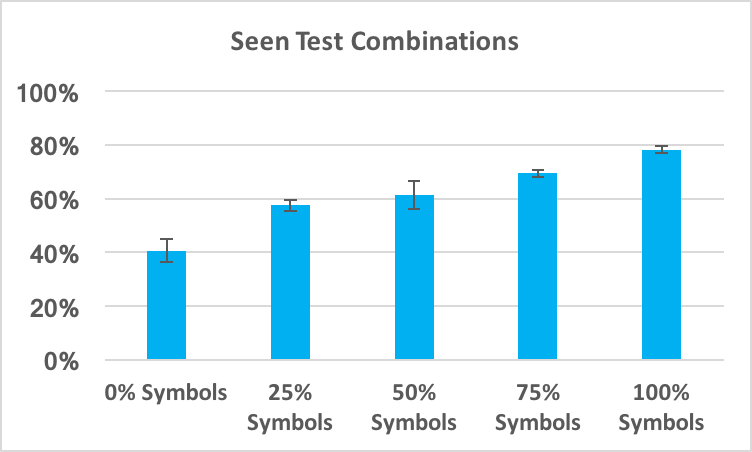
\includegraphics[width=0.5\textwidth]{experiment-4-results-chart-seen}}}%
	\subfloat[Unseen Test Combinations]{{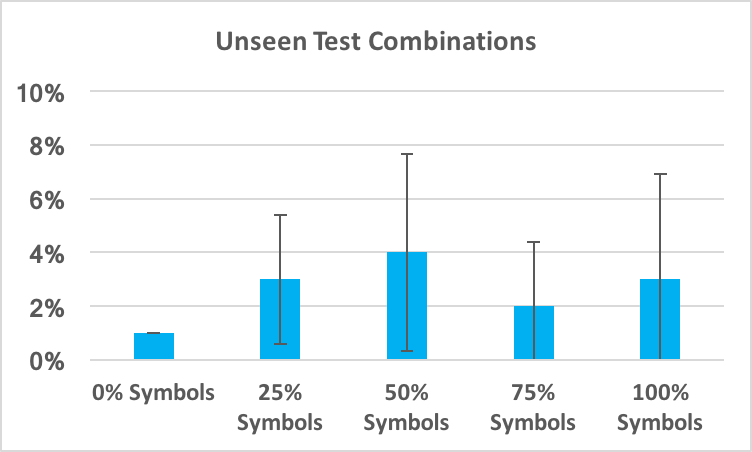
\includegraphics[width=0.5\textwidth]{experiment-4-results-chart-unseen}}}%
	\caption{A comparison of the mean accuracy and 95\% confidence intervals for each of the models when tested on both the \textbf{seen} and \textbf{unseen} test combinations.}
	\label{fig:experiment-4-results-chart}
\end{figure}

Table \ref{tab:experiment-4-results-table-seen} shows the mean accuracy, standard deviation and t-test p-value scores for the test set which uses the same operand combinations that the models were trained on. Table \ref{tab:experiment-4-results-table-unseen} shows these same metrics when the same models are tested on operand combinations they have never seen before. Figure \ref{fig:experiment-4-results-chart} shows graphs of these results along with 95\% confidence intervals.

Table \ref{tab:experiment-4-results-table-seen} shows similar accuracies to those obtained in Experiment 2 with the models trained in the presence of symbols outperforming the ones trained without symbols. However, the models when tested on the unseen dataset show poor performance regardless of whether they are trained with symbols or not.

\subsubsection{Discussion}

It is clear from these results that the current recurrent neural network models are unable to generalize to unseen combinations of operands. They are unable to discover a representation for an algorithm for the arithmetic operations. The models perform well on the previously experienced combinations by developing a sequential mapping function for those seen operand combinations.

In the next section, we describe an experiment that examines our theory in Section \ref{sec:theory-approach-methodology-pattern-matching-vs-learning-an-algorithm} to understand how this pattern matching works and how the presence of symbols makes this process more effective. Later, we present a different approach that uses a modified representation of the symbols as discussed in Section \ref{sec:theory-approach-methodology-temperature-encoding}. Using this new representation, we are able to develop a model that performs well on unseen test sets.